\documentclass{article}
\usepackage{hyperref}
\usepackage{graphicx}
\usepackage{subcaption}
\usepackage{amssymb}
\usepackage{titlesec}
\usepackage{xcolor, soul}
\usepackage{amsmath}
\usepackage{amsfonts}
\usepackage{cancel}
\usepackage{minted}
\usepackage{apacite}
\usepackage{caption}
\usepackage{cleveref}
\usepackage{tcolorbox}
\usepackage{float}
\usepackage{pdfpages}
\usepackage{tabularx}
\setlength{\parindent}{0pt}
\usepackage[margin=0.9in]{geometry}

\hypersetup{
colorlinks   = true,    % Colours links instead of ugly boxes
urlcolor     = blue,    % Colour for external hyperlinks
linkcolor    = blue,    % Colour of internal links
citecolor    = blue      % Colour of citations
}
\usepackage{enumitem,amssymb}
\newlist{todolist}{itemize}{2}
\setlist[todolist]{label=$\square$}

\sethlcolor{yellow}



\setcounter{secnumdepth}{4}
\setlength{\parskip}{7pt} % paragraph spacing
\let\oldmarginpar\marginpar
\renewcommand\marginpar[1]{\oldmarginpar{\tiny #1}} % Change "small" to your desired font size]
\begin{document}
\date{}
\author{Marios Gkionis}
\title{e}
\maketitle

\tableofcontents 
 \newpage

\section{Development Tasks}


% Start obsidian ref:
%dev-tasks
\begin{todolist}
\item Allow user to create more complex configurations
\item Tables
\begin{todolist}
\item Use the QuickAdd logic for tables
\item Allow user to modify the column widths from Obsidian
\item Allow entries be empty
\item Fancy formatting
\end{todolist}
\item Allow the user to change settings from Obsidian, instead of Python
\end{todolist}
% End obsidian ref


\section{Formatting}




% Start obsidian ref:
%formatting
\textit{italic text}

\textbf{bold text}

\hl{highlighted text}

% End obsidian ref




\section{Itemization}

\subsection{Bullet list}

\begin{itemize}
\item Item 1
\begin{itemize}
\item item 1.1
\item item 1.2
\begin{itemize}
\item item 1.2.1
\end{itemize}
\end{itemize}
\item Item 2
\begin{enumerate}
\item Enumeration 1
\begin{enumerate}
\item Enumeration 1.2
\item Enumeration 2.2
\end{enumerate}
\item Enumeration 2
\begin{enumerate}
\item Enumeration 2.1
\begin{itemize}
\item Bullet 2.1.1
\end{itemize}
\end{enumerate}
\item Enumeration 3
\end{enumerate}
\end{itemize}


\subsection{Enumerated list}

\begin{enumerate}
\item Item 1
\item Item 2
\begin{enumerate}
\item Item 2.1
\item Item 2.2
\end{enumerate}
\end{enumerate}


\subsection{Task list}

\begin{todolist}
\item Task 1
\item Task 2
\item Task 3
\begin{todolist}
\item Task 3.1
\end{todolist}
\item Task 4
\end{todolist}
\section{Adding citations} \label{sec:Adding-citations}

Command: just mention that link that pertains to the literature file. I use the "p"+"number" naming convention. For example, "p1" would be the first literature file in my vault.



Example: In \cite{p1}, we see that...  \hypertarget{ad3b86}{} \label{ead3b86}



\section{Equations}

Both equations and subfigures are written in the form of embedded notes, since they are encoded as notes.

\subsection{Writing the equation}



Steps:



\begin{enumerate}
\item Press ctrl+P, then Quickadd: equation\_block\_single
\end{enumerate}



% Start obsidian ref:
%eq__block_Einsteinexpr
\begin{equation} \label{eq:Einstein}
	E=mc^{2}
\end{equation}

% End obsidian ref




It supports the aligned equations, as seen in \cref{eq:1}.




% Start obsidian ref:
%eq__block_1expr
\begin{equation}\label{eq:1}
\begin{aligned}
\Delta W_{rg} = -\alpha \sum_{s}&[R+\gamma V(s')-V(s)]  \\
&[\nabla_{w} \gamma V(s')-\nabla_{w}V(s)]
\end{aligned}
\end{equation}

% End obsidian ref


\subsection{Referencing the equation}

In \cref{eq:Einstein}, we see that...

\section{Figures}

\subsection{Adding figures}

\subsubsection{No subfigures}


% Start obsidian ref:
%figure__block_gradient_stepsfig
\begin{figure}[H]
\centering
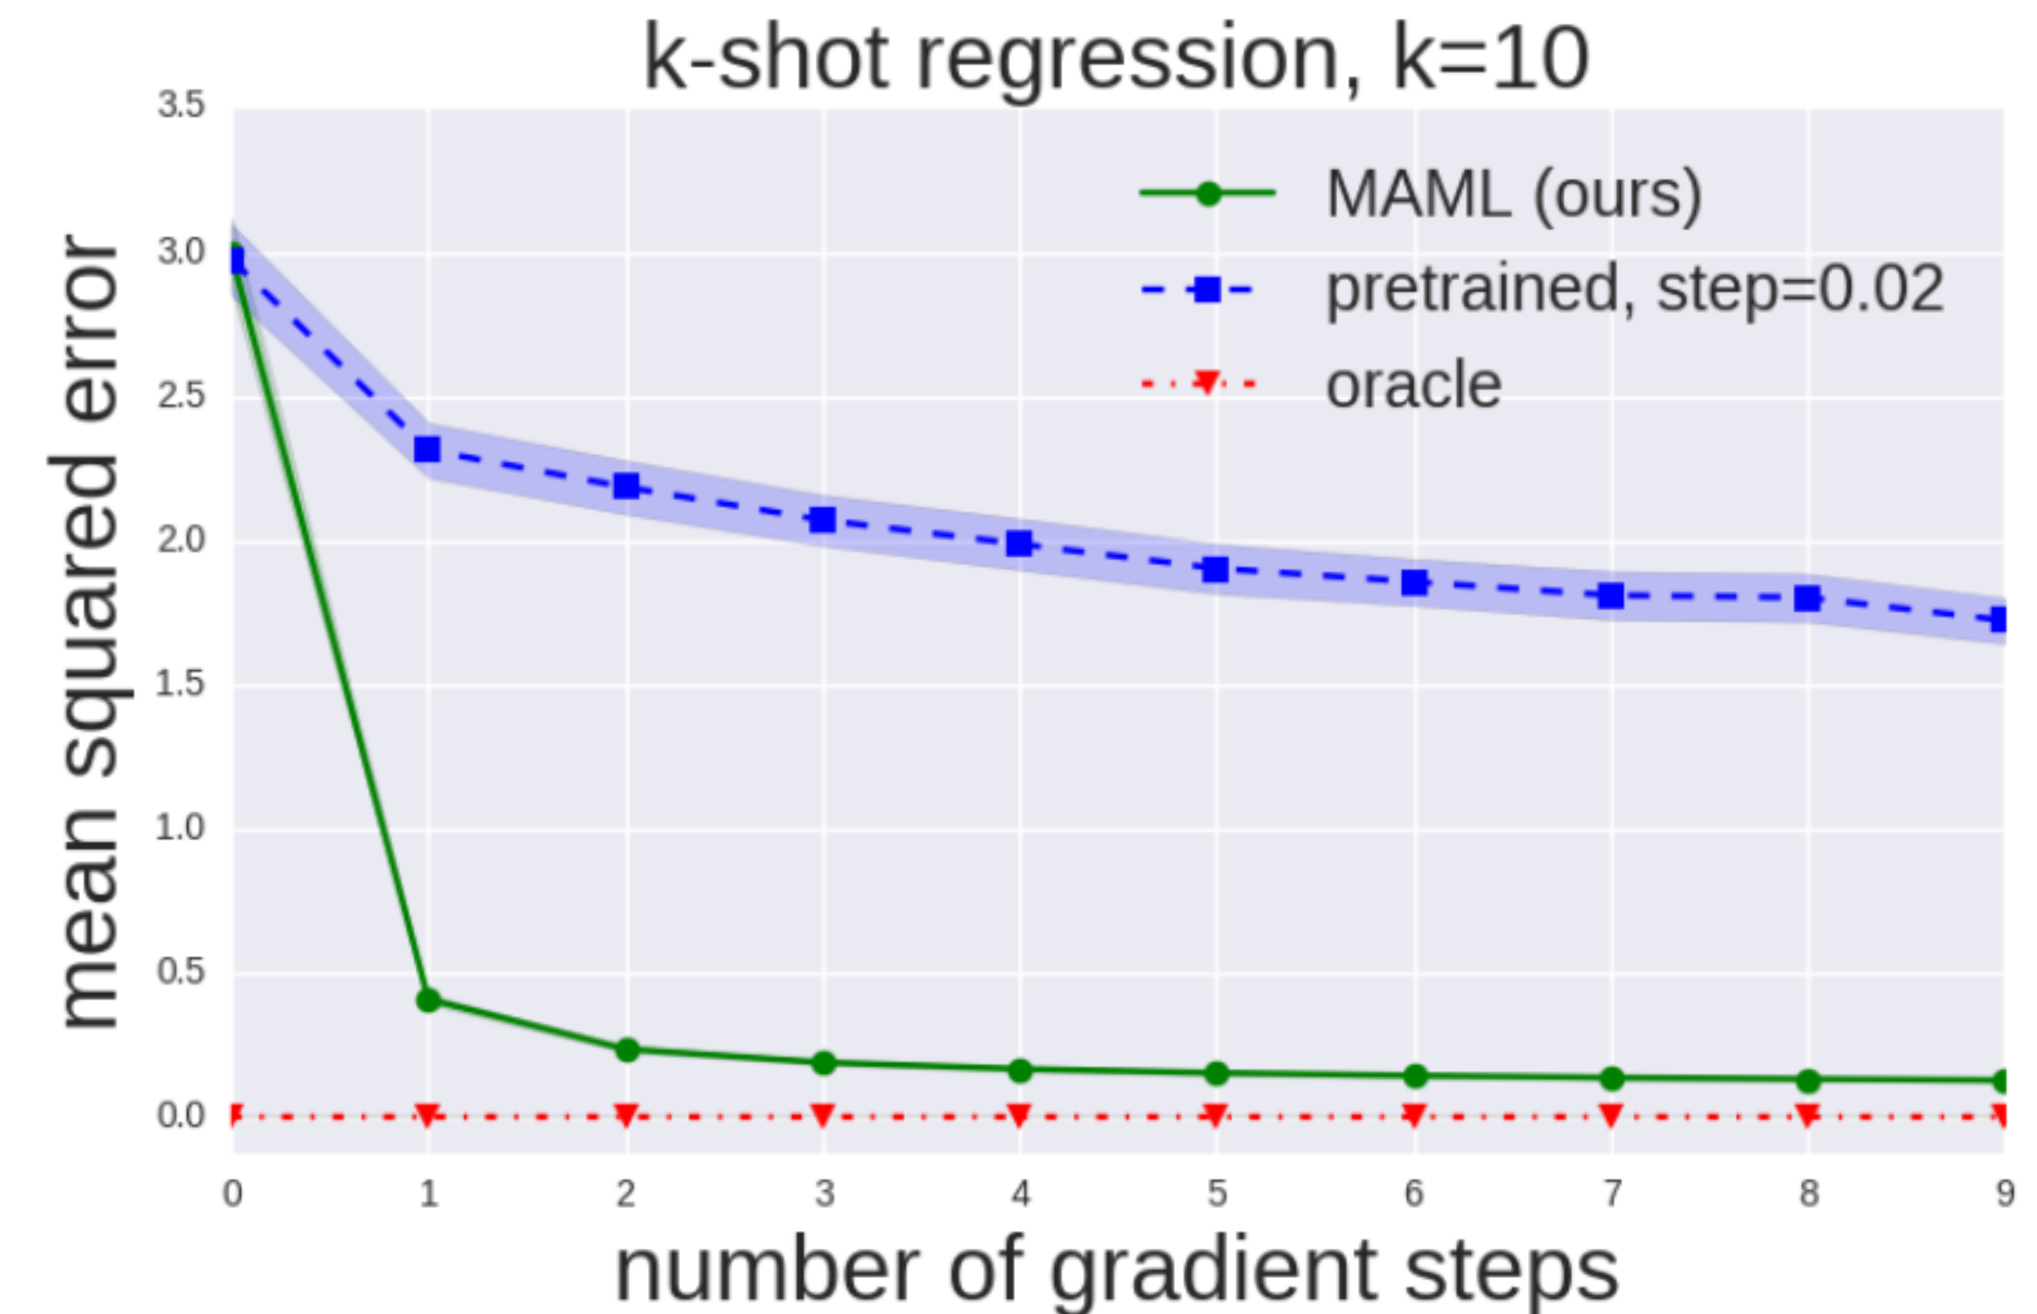
\includegraphics[width=0.4\linewidth]{"C:/Users/mariosg/OneDrive - NTNU/FILES/workTips/Literature/Straightforward-Obsidian2Latex/example_vault/✍Writing/figure blocks/Pasted image 20240609012140.png"}
\caption[]{The caption.}

\label{fig:gradient_steps}
\end{figure}
% End obsidian ref




\subsubsection{With subfigures}

\begin{itemize}
\item \textbf{TODO: }  Allow user to create more complex configurations
\end{itemize}

% Start obsidian ref:
%figure__block_1fig
\begin{figure}[H]
\centering
\begin{subfigure}[b]{0.5\textwidth}
\centering
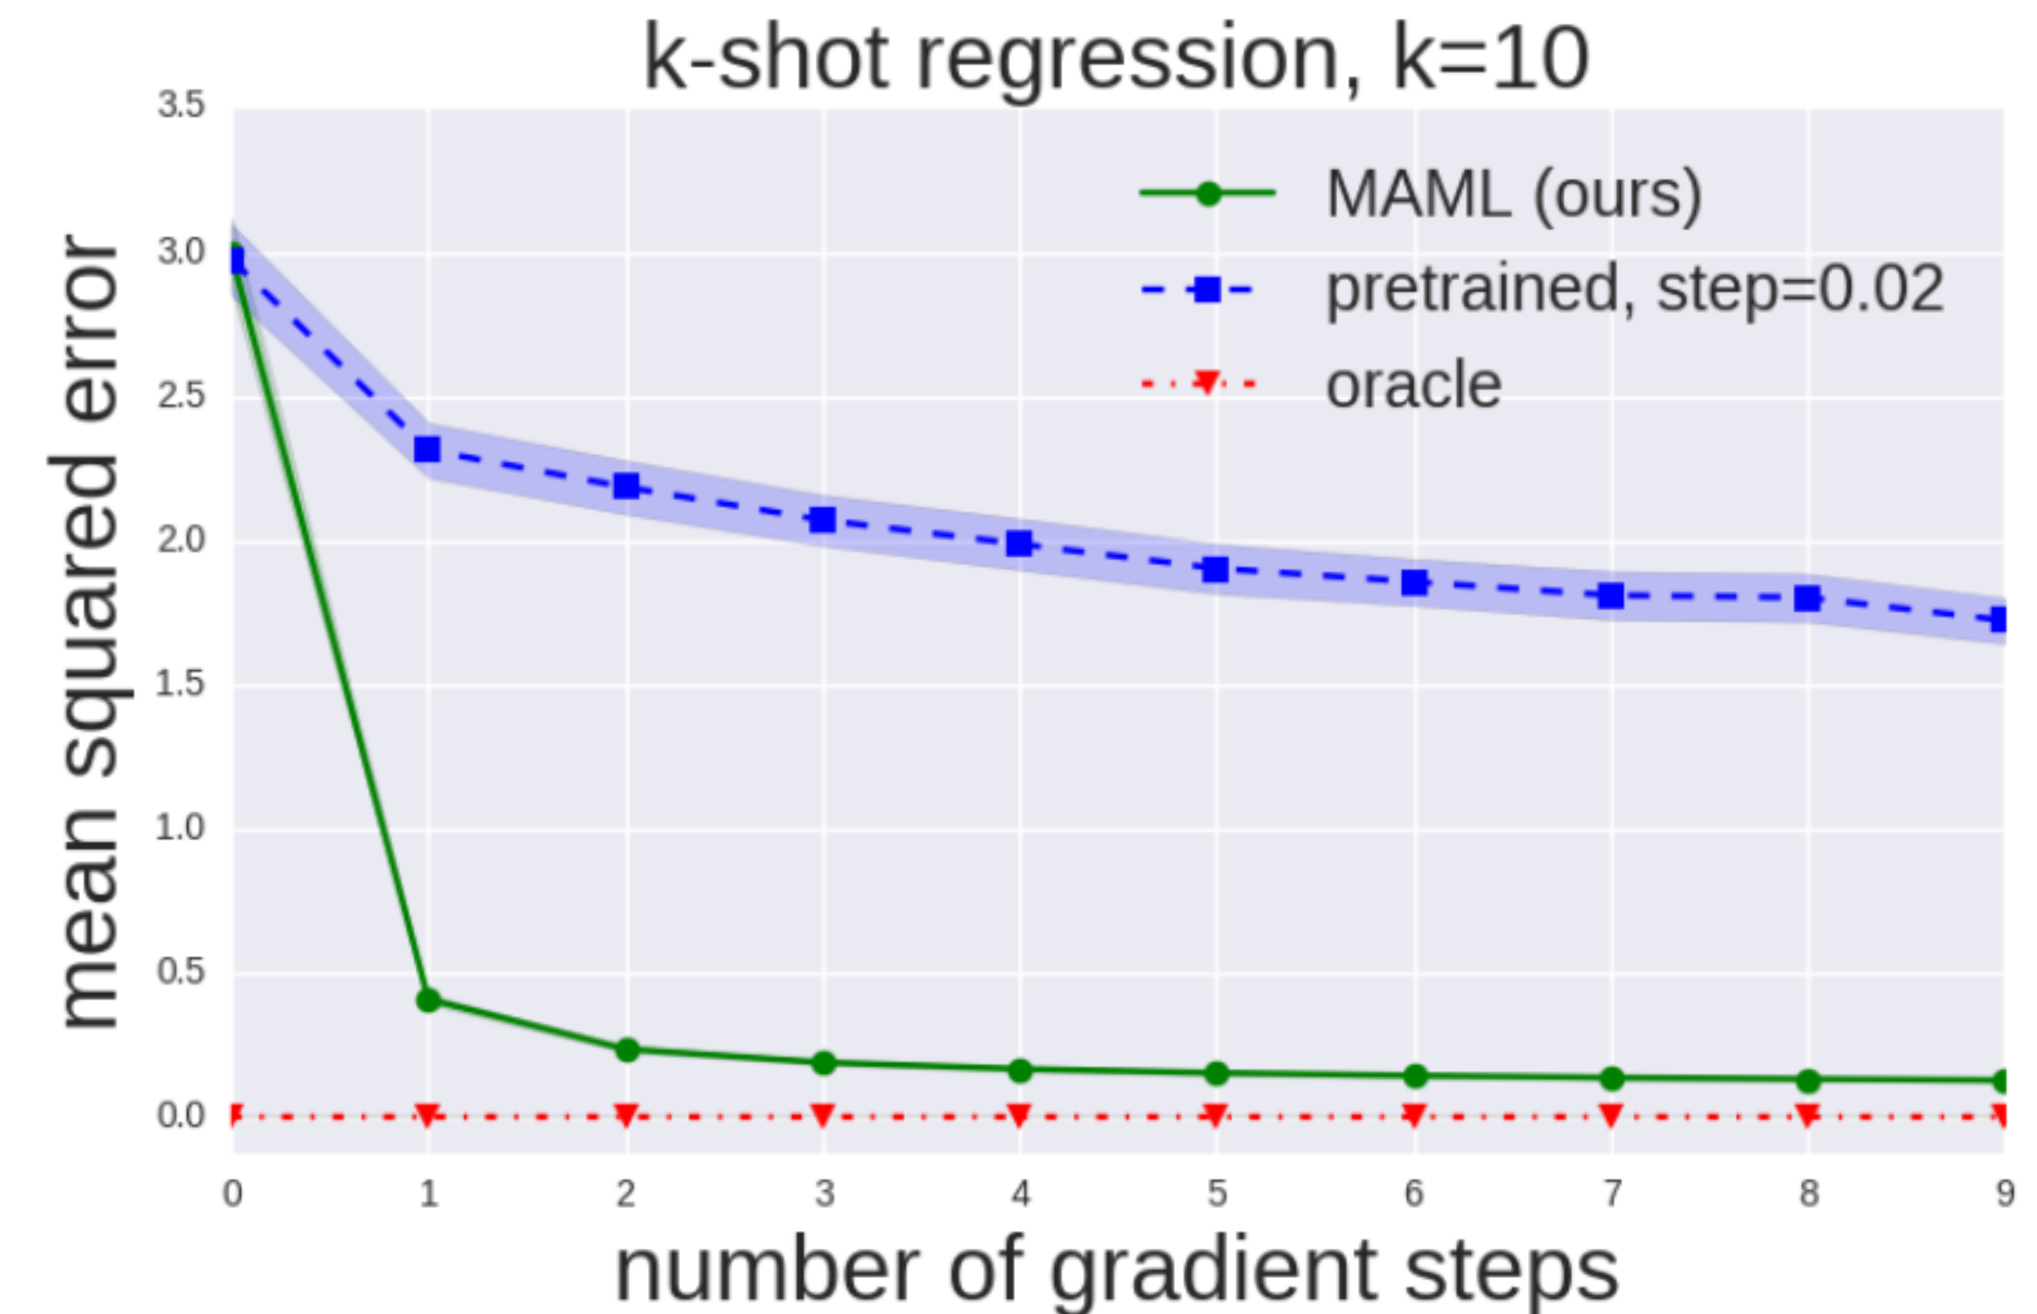
\includegraphics[width=\linewidth]{"C:/Users/mariosg/OneDrive - NTNU/FILES/workTips/Literature/Straightforward-Obsidian2Latex/example_vault/✍Writing/figure blocks/Pasted image 20240609012221.png"}
\caption[]


\end{subfigure}\hfill
\begin{subfigure}[b]{0.5\textwidth}
\centering
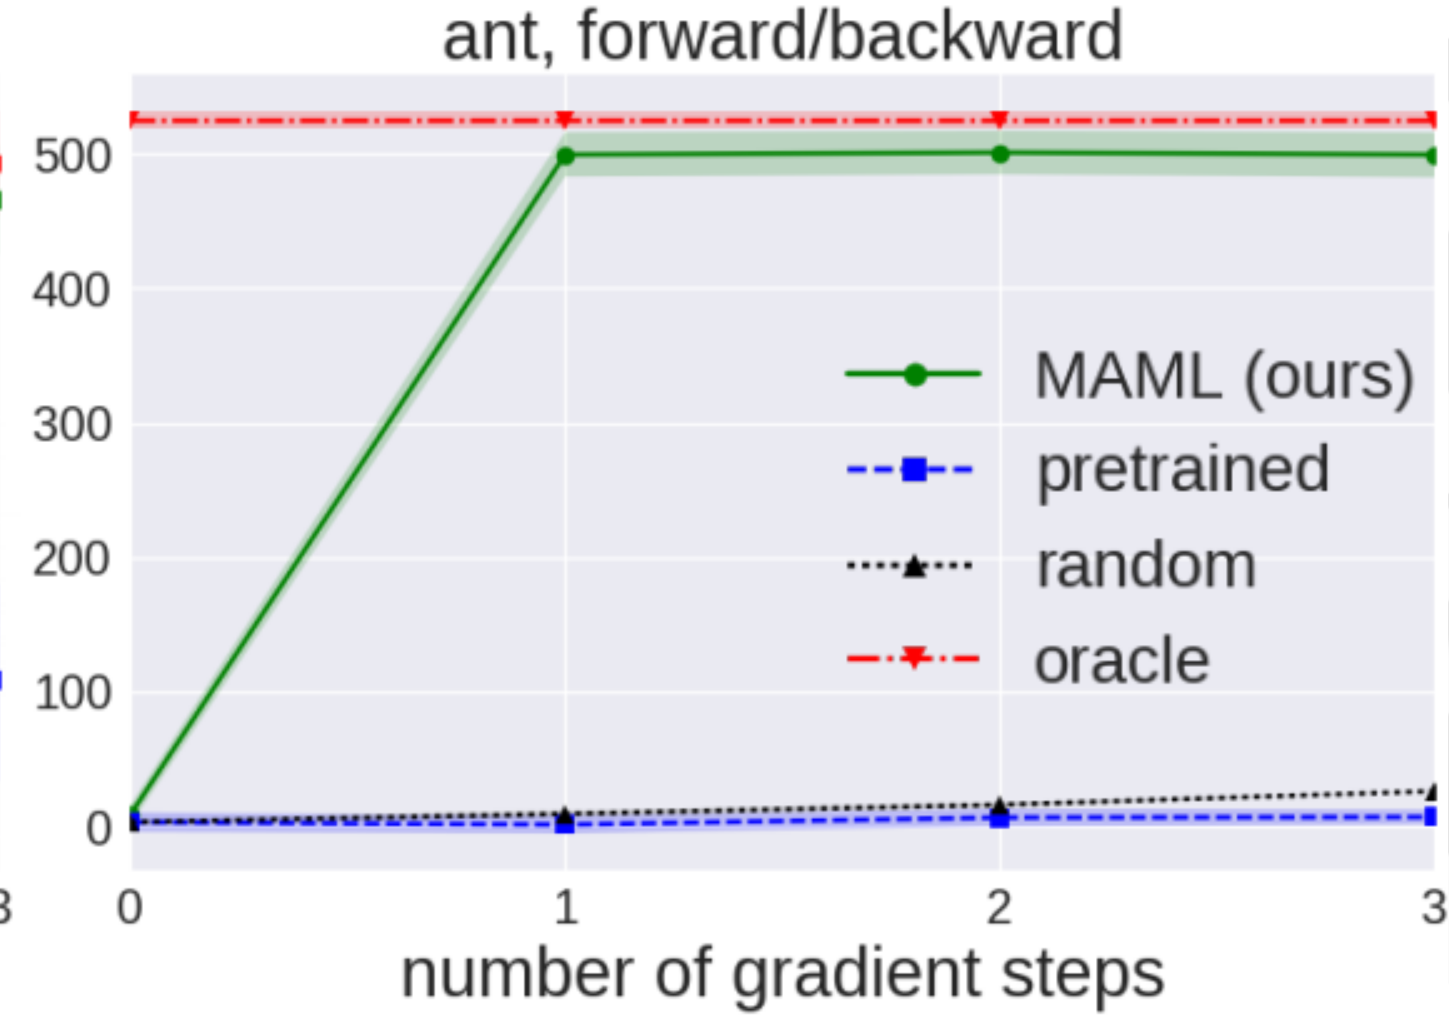
\includegraphics[width=\linewidth]{"C:/Users/mariosg/OneDrive - NTNU/FILES/workTips/Literature/Straightforward-Obsidian2Latex/example_vault/✍Writing/figure blocks/Pasted image 20240609012251.png"}
\caption[]


\end{subfigure}\hfill
\caption{}
\label{fig:1}
\end{figure}

% End obsidian ref






\subsection{Referencing figures}

In \cref{fig:1}, we can notice that...





\section{Admonition blocks}

If you write admonition blocks, they are translated into something similar in latex.

\textbf{Example}

\begin{tcolorbox}[width=\textwidth,colback={red},title={warning},outer arc=0mm,colupper=white]

This is a warning

\end{tcolorbox}



\begin{tcolorbox}[width=\textwidth,colback={white},title={note},outer arc=0mm,colupper=black]

This is a note

\end{tcolorbox}





\section{Code blocks}

\begin{minted}{python}

print("this is a code block")

print("this is another code block")

\end{minted}



\section{Cross-reference of section}

Check \hyperref[sec:Adding-citations]{this section}: \autoref{sec:Adding-citations} about adding citations.





\section{\maltese Cross-reference of block}

example



\section{Assume sections from embedded notes}

The sections from embedded notes can assume the hierarchy of the file wherein they are embedded.

\begin{tcolorbox}[width=\textwidth,colback={white},title={note},outer arc=0mm,colupper=black]

Notice in the latex file that the section hierarchy has been modified to adhere to the hierarchy of the file that embeds the note.

\end{tcolorbox}




% Start obsidian ref:
%embedded with sections
\subsection{Section 1 of embedded}
\subsubsection{subsection 1 of embedded}
% End obsidian ref




\section{Hyperlinks}

Click \href{https://www.youtube.com/}{here}.





\section{Tables}



\newcolumntype{Y}{>{\centering\arraybackslash}X}
\renewcommand\tabularxcolumn[1]{m{#1}}
\begin{center}
\begin{tabularx}{\textwidth}{|Y|Y|Y|Y|}
   \hline
    \textbf{Col1} & \textbf{Col2} & \textbf{Col3} & \textbf{Col4} \\ \hline
    a11 & a12 & Some more text & even more text \\ \hline
    a21 & Equation: $E=mc^{2}$ & Some more textSome more textSome more textSome more textSome more textSome more text & even more text even more text even more text even more text even more text \\ \hline
    Reference \cref{eq:1} & 1 & 1 & 1 \\ \hline
   \hline
\end{tabularx}
\end{center}
\newpage 
 \bibliographystyle{apacite}
\bibliography{BIBTEX}
\end{document}
